
\begin{figure}
	\centering
   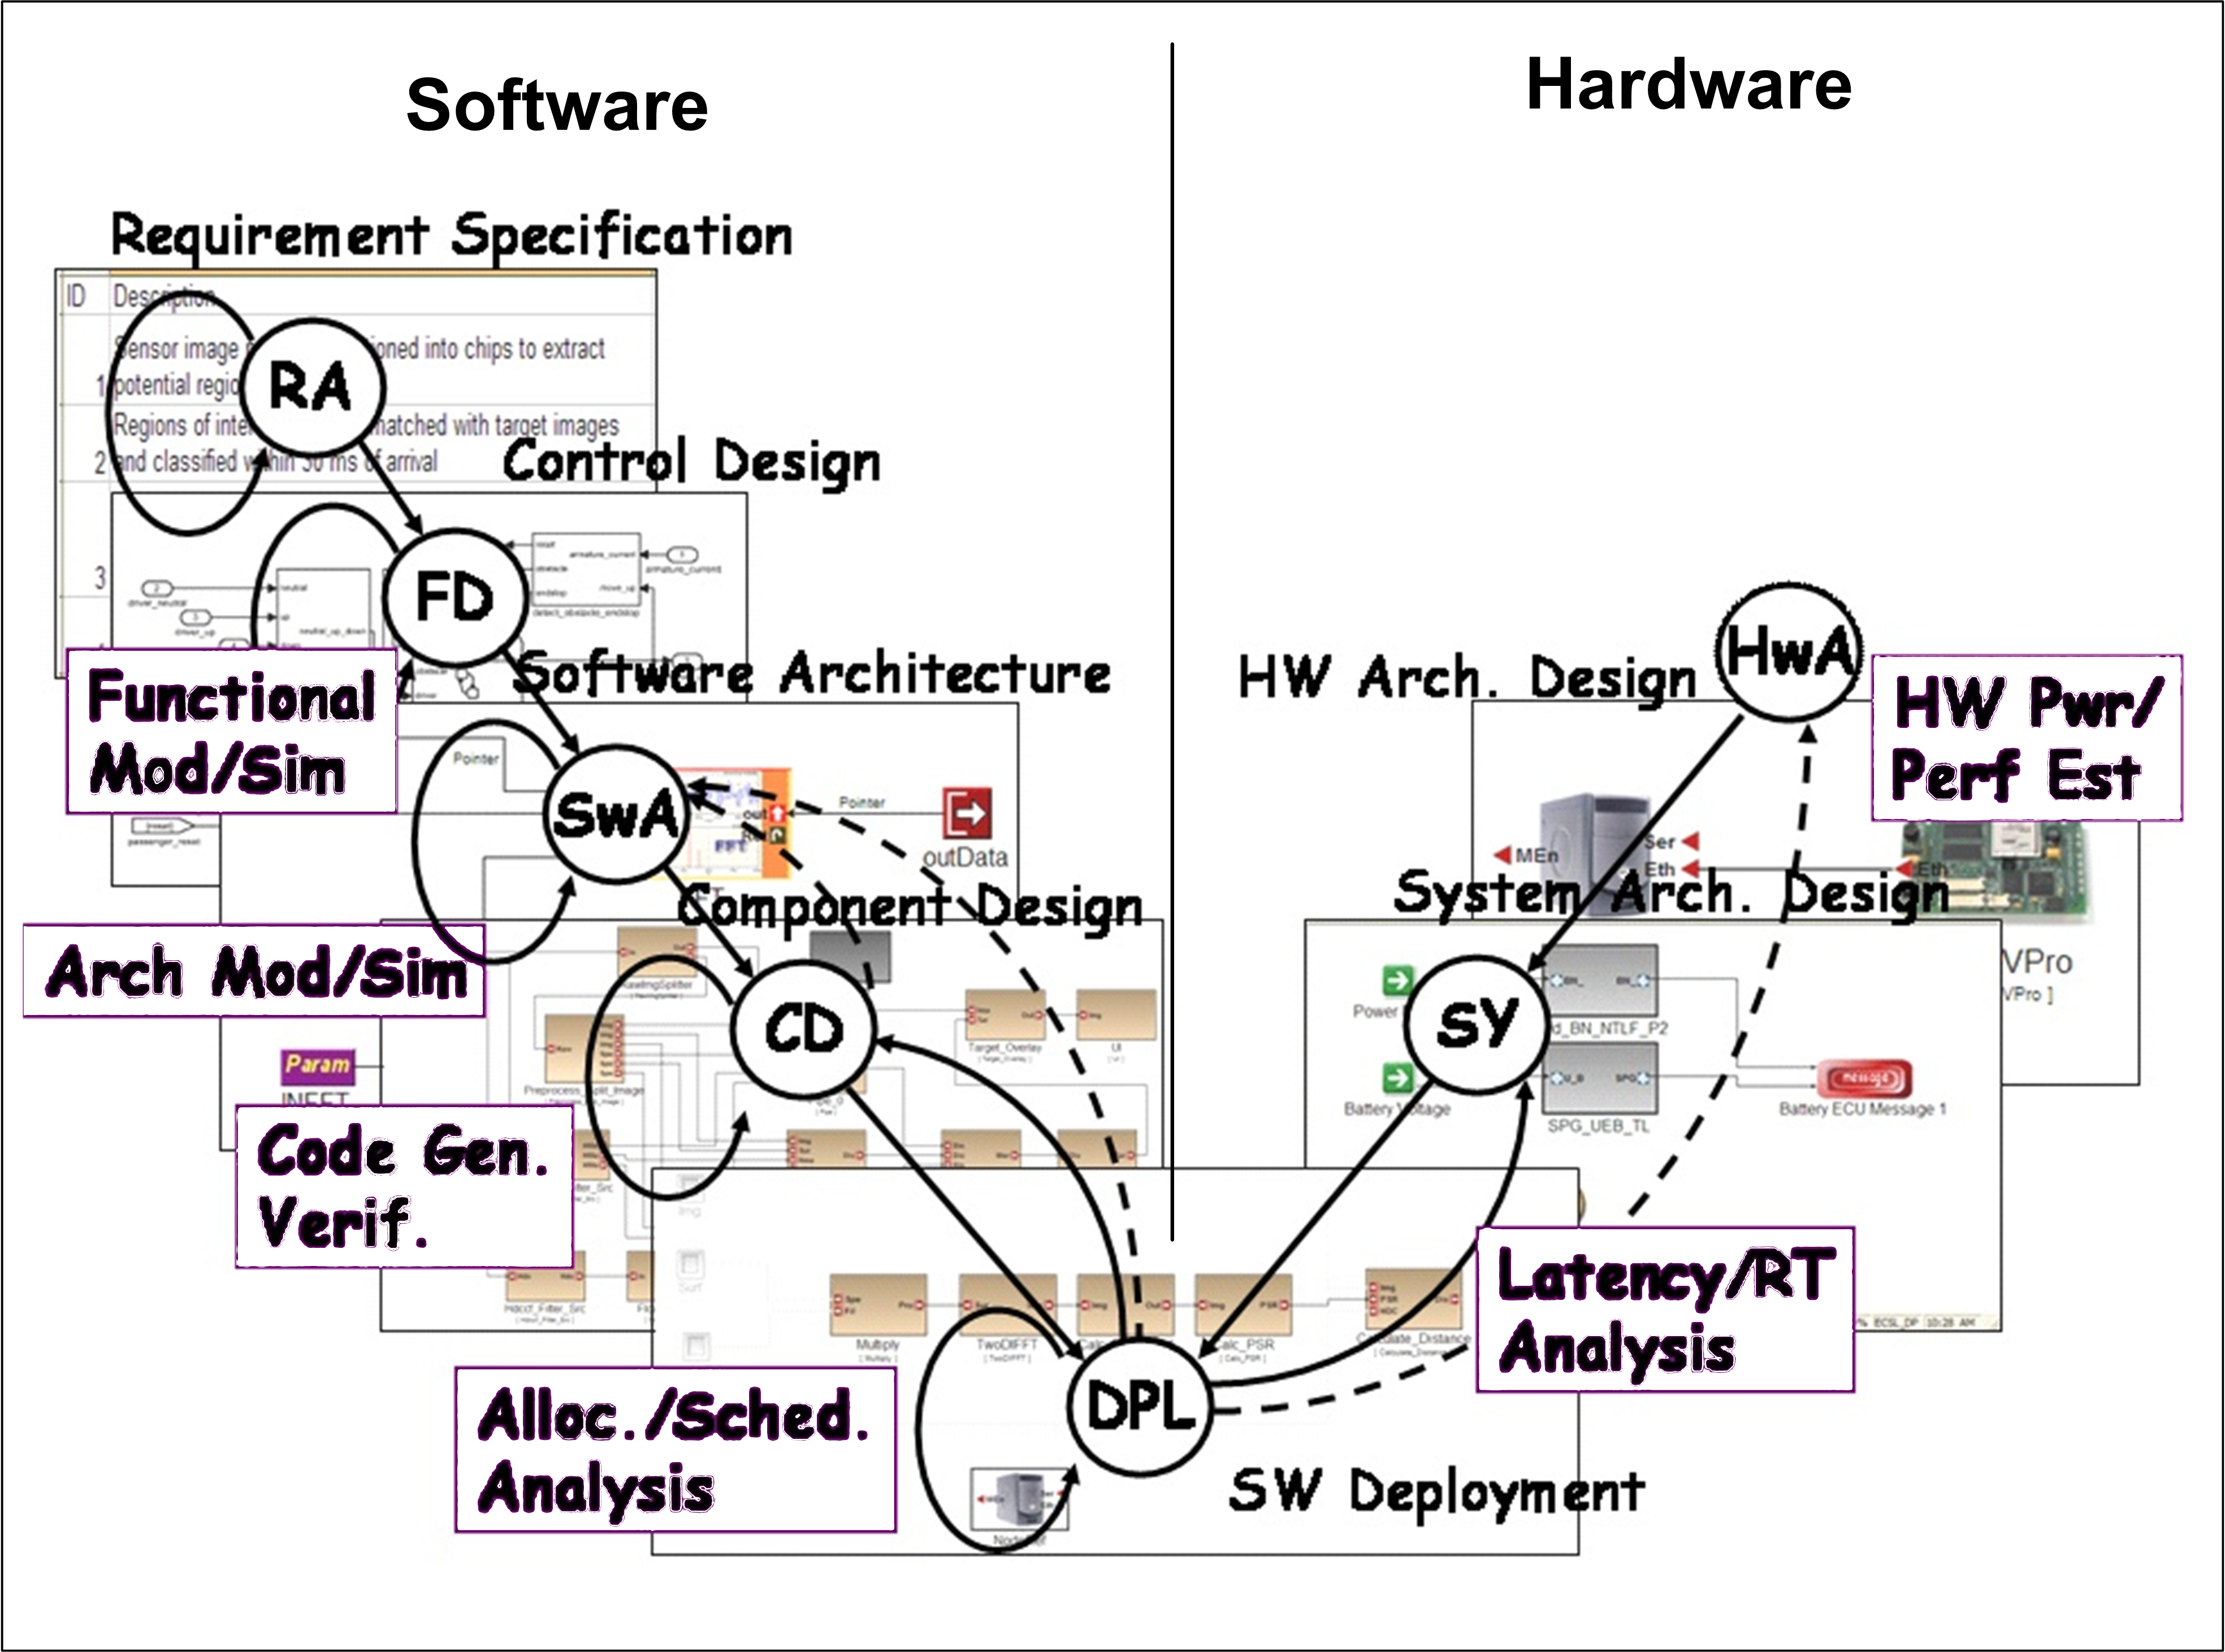
\includegraphics[width=0.65\columnwidth]{diagrams/vdiagram.png}
   \caption{Conceptual model of the toolchain: Development flow}
   \label{fig:vdiagram}
\end{figure}

In this work, we envision a sophisticated, end-to-end toolchain that supports not only construction but also the verification of the engineering artifacts (including software) for high-confidence applications. The development flow provided by the toolchain shall follow a variation of the classical V-model (with software and hardware development on the two branches), with some refinements added at the various stages. Fig. \ref{fig:vdiagram} illustrates this development flow.

Consider the general class of control system designs for use in a flight control system.  Sensors, actuators, and data networks are designed redundantly to mitigate faults.  The underlying hardware implements a variant of the time-triggered architecture (TTA)~\cite{kopetz:2001-22a}, which provides precise timing and reliability guarantees.  Safety-critical tasks and messages execute according to strict precomputed schedules to ensure synchronization between replicated components and provide fault mitigation and management.  Software implementations of the control functions must pass strict certification requirements which impose constraints on the software as well as on the development process.  

A modeling language to support this development flow must have several desired properties:  (1) the ability to capture the relevant aspects of the system architecture and hardware, (2) ability to ``understand'' (and import) functional models from existing design tools, (3) support for componentization of functional models, and (4) ability to model the deployment of the software architecture onto the hardware architecture. The ability to import existing models from functional modeling tools is not a deeply justified requirement, it is merely pragmatic.  EsMoL provides modeling concepts and capabilities that are highly compatible with AADL~\cite{AADL}.  The chief differences are that EsMoL aims for a simpler graphical entry language, a wider range of execution semantics, and most important model-enabled integration to external tools as described below.  Model exchange with AADL tools may be desirable in the future.  A simple sample design will introduce key points of our model-based development flow and illustrate language concepts.  

Our language design was influenced by two factors: (1) the MoC implemented by the platform and (2) the need for integration with legacy modeling and embedded systems tools. We have chosen Simulink/Stateflow as the supported ``legacy'' tool. As our chosen MoC relies on periodically scheduled time-triggered components, it was natural to use this concept as the basis for our modeling language and interpret the imported Simulink blocks as the implementation of these components. To clarify the use of this functionality, we import a Simulink design and select functional subsets which execute in discrete time, and then assign them to software components using a modeling language that has compatible (time-triggered) semantics. Communication links (signals) between Simulink blocks are mapped onto TTA messages passed between the tasks. The resulting language provides a componentized view of Simulink models that are scheduled periodically (with a fixed rate) and communicate using time-triggered messages.  Extensions to heterogeneous MoC-s is an active area of research.

\subsection{Requirements Analysis (RA)}

Our example will model a data network implementing a single sensor/actuator loop with a distributed implementation.  The sensors and actuators in the example are doubly-redundant, while the data network is triply-redundant.  Unlike true safety-critical designs, we will deploy the same functions on all replicas rather than requiring multiple versions as is often done in practice~\cite{DO178B}.  The sensors and actuators close a single physical feedback loop.  Specifying the physical system and particulars of the control functions are beyond the scope of this example as our focus is on modeling.

This example has an informal set of requirements, though our modeling language currently supports the formalization of timing constraints between sensor and actuator tasks.  Formal requirements modeling offers great promise, but in ESMoL requirements modeling is still in conceptual stages.  A simple sensor/actuator latency modeling example appears in a later section covering preliminary features for the language.

\subsection{Functional Design (FD)}

\begin{figure}
	\centering
   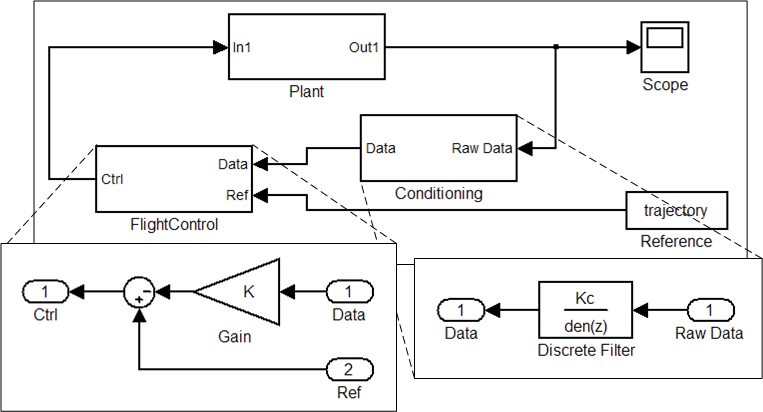
\includegraphics[width=0.65\columnwidth]{diagrams/sl_design.png}
   \caption{Simulink design of a basic signal conditioner and controller.}
   \label{fig:sl_design}
\end{figure}

Functional designs can appear in the form of Simulink/Stateflow models or as existing C code snippets.  ESMoL does not support the full semantics of Simulink. In ESMoL the execution of Simulink data flow blocks is restricted to periodic discrete time, consistent with the underlying time-triggered platform.  This also restricts the type and configuration of blocks that may be used in a design.  Continuous integrator blocks and sample time settings do not have meaning in ESMoL.  C code snippets are captured in ESMoL as well.  C code definitions are limited to synchronous, bounded-time function calls which will execute in a periodic task.

\begin{figure}
	\centering
   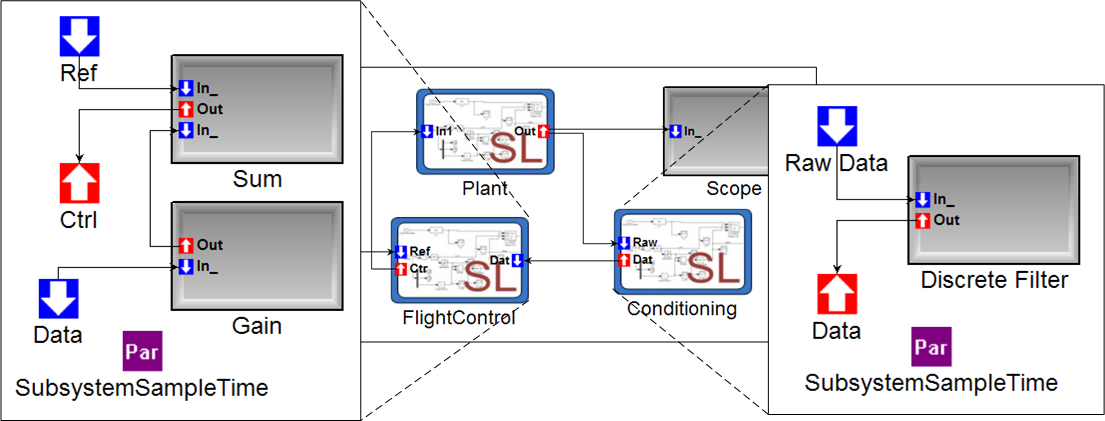
\includegraphics[width=0.9\columnwidth]{diagrams/esmol_design.png}
   \caption{ESMoL-imported functional models of the Simulink design.}
   \label{fig:esmol_design}
\end{figure}

Fig. \ref{fig:sl_design} shows a simple top-level Simulink design for our feedback loop along with the imported ESMoL model (Fig. \ref{fig:esmol_design}).  The ESMoL model is a structural replica of the original Simulink, only endowed with a richer software design environment and tool-provided APIs for navigating and manipulating the model structure in code.  A model import utility provides the illustrated function.

\subsection{Software Architecture (SwA)}

\begin{figure}
	\centering
   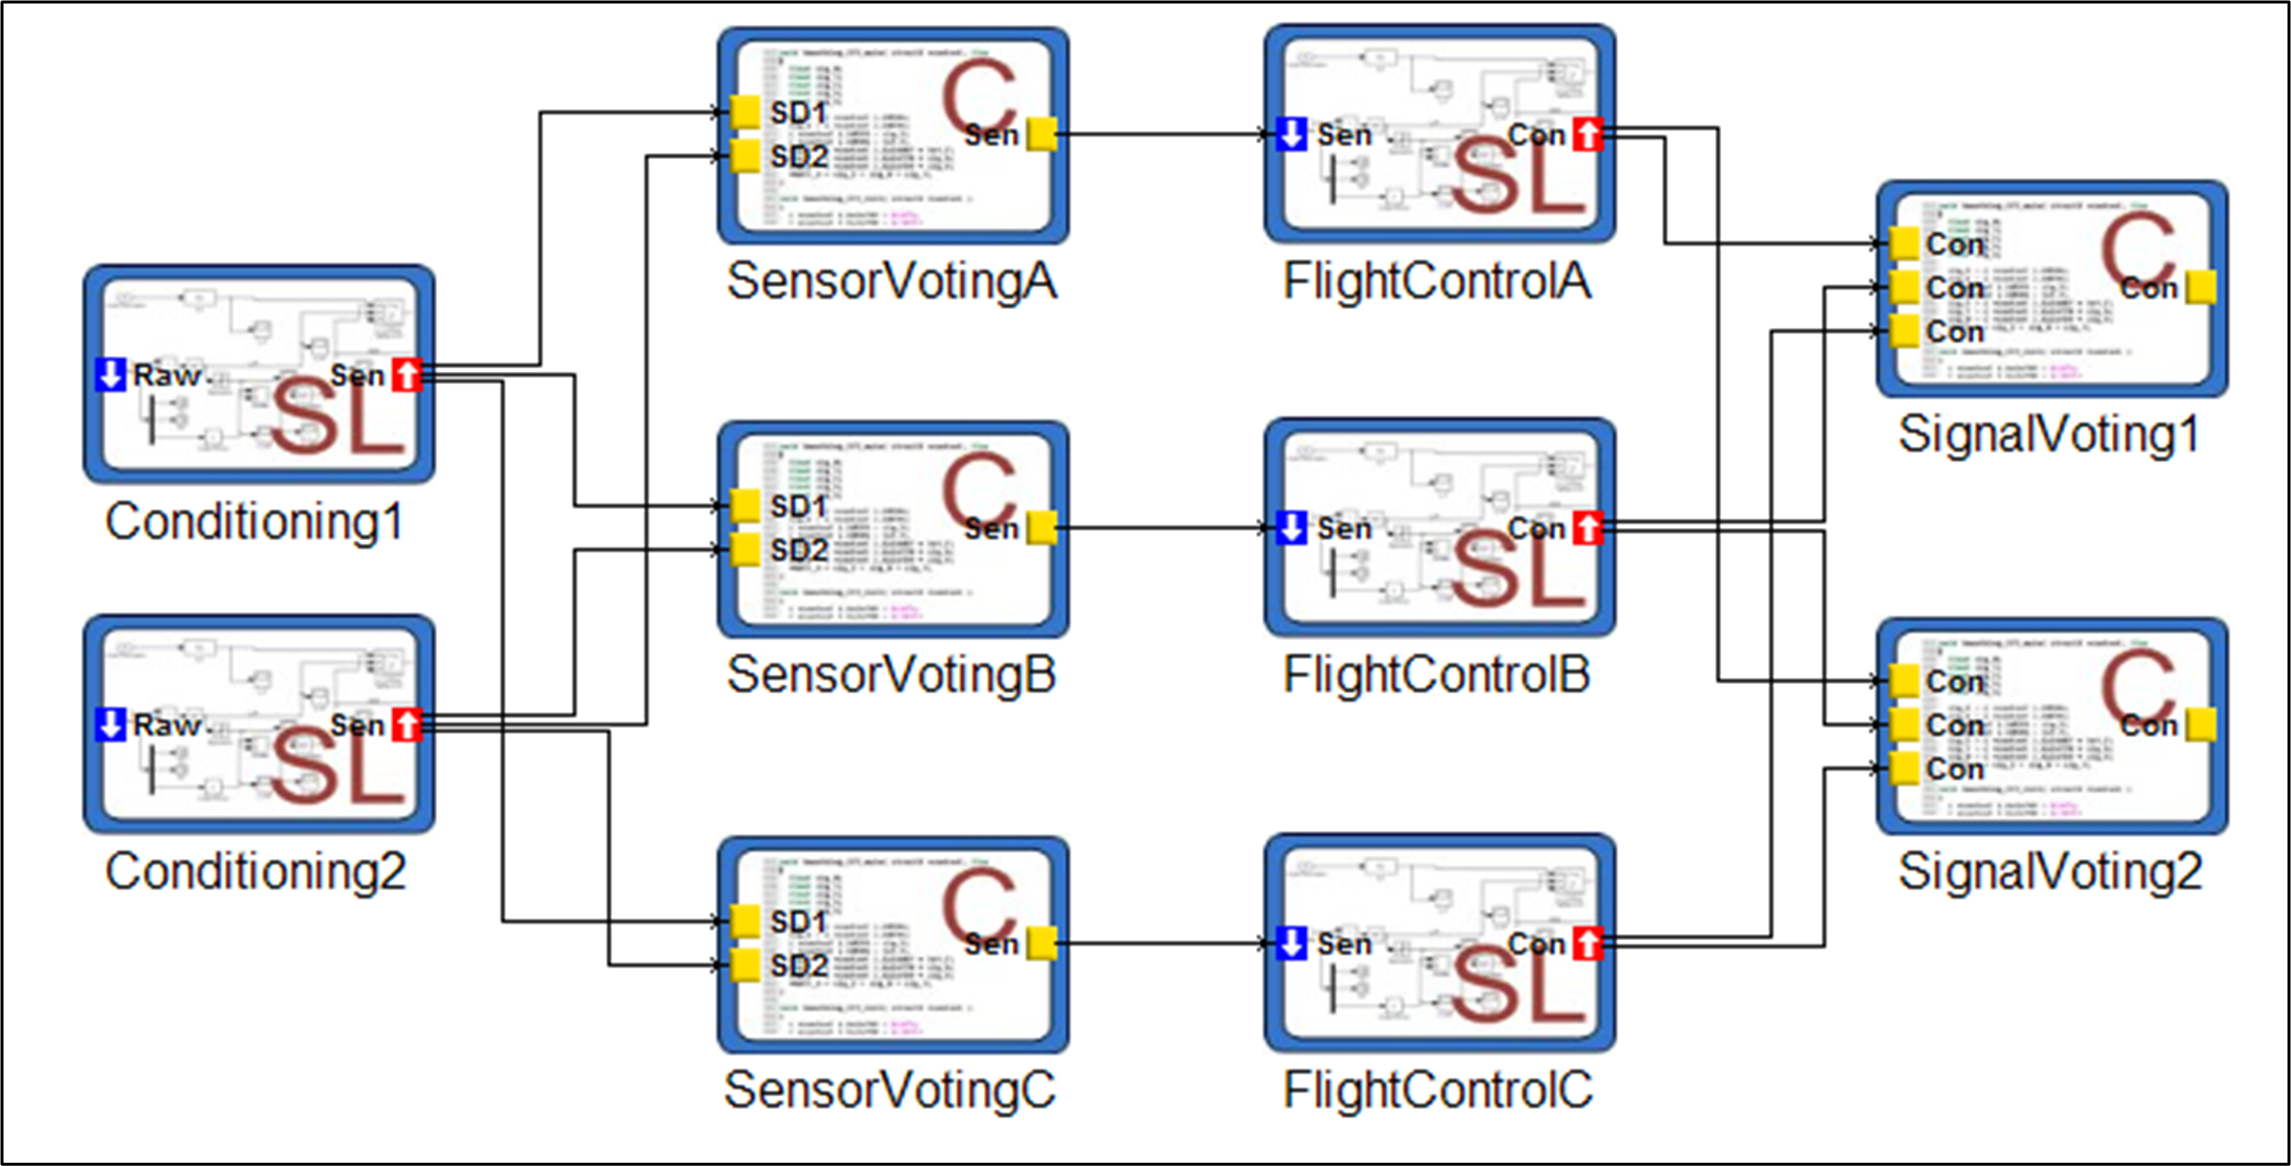
\includegraphics[width=0.7\columnwidth]{diagrams/tmr_arch.png}
   \caption{The architecture diagram defines logical interconnections, and gives finer control over instantiation of functional units.}
   \label{fig:tmr_arch}
\end{figure}

The software architecture model describes the logical interconnection of functional blocks.  In the architecture language a component may be implemented by either a Simulink Subsystem or a C function.  They are compatible at this level, because here their model elements represent the code that will finally implement the functions.  These units are modeled as blocks with ports, where the ports represent parameters passed into and out of C function calls.  The semantics for architecture model connections is that of sending and receiving messages using time-triggered communication.  

Fig. \ref{fig:tmr_arch} shows the architecture diagram for our TMR model.  Instances of the functional blocks from the Simulink model are augmented with C code implementing replicated data voting.

\subsection{Hardware Architecture (HwA)}

\begin{figure}
	\centering
   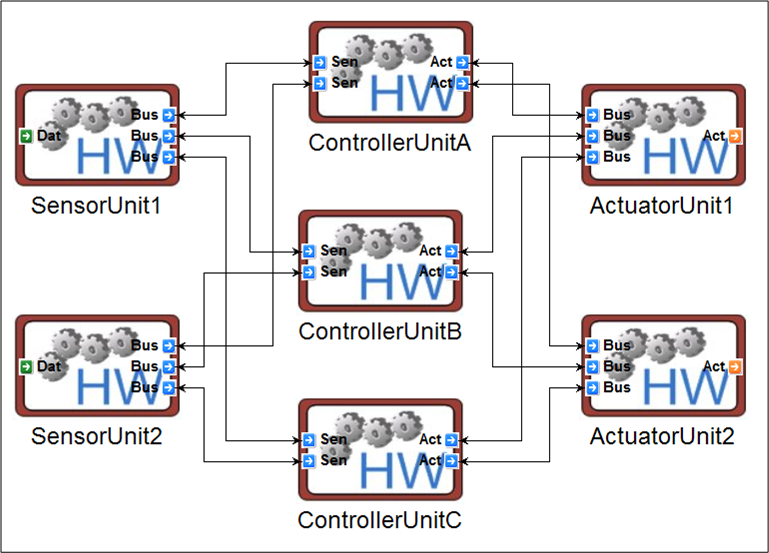
\includegraphics[width=0.75\columnwidth]{diagrams/tmr_hardware.png}
   \caption{Overall hardware layout for the TMR example.}
   \label{fig:tmr_hardware}
\end{figure}

Hardware configurations are explicitly modeled in the platform language.  Platforms are defined hierarchically as hardware units with ports for interconnections. Primitive components include processing nodes and communication buses.  Behavioral semantics for these networks come from the underlying time-triggered architecture.  The platform provides services such as deterministic execution of replicated components and timed message-passing.  Model attributes for hardware also capture timing resolution, overhead parameters for data transfers, and task context switching times.

\begin{figure}
	\centering
   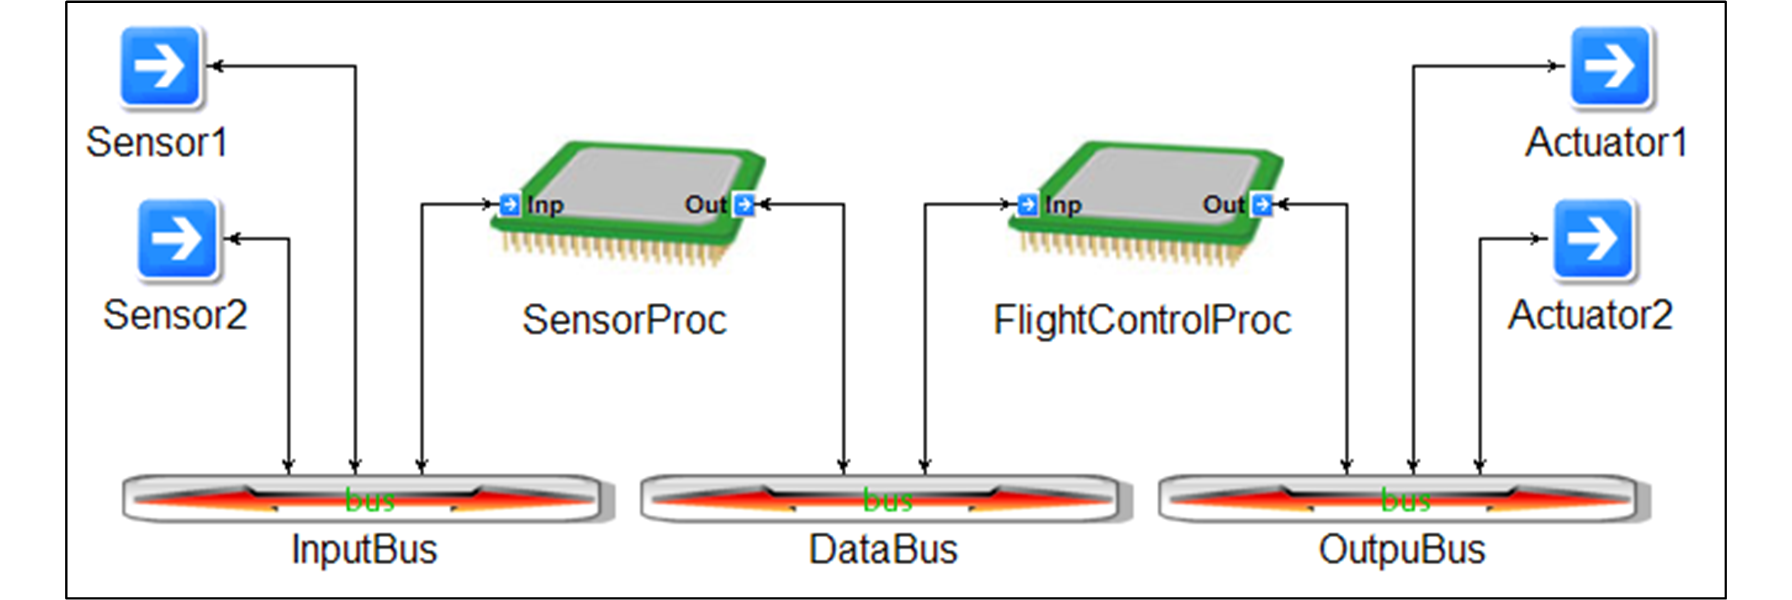
\includegraphics[width=0.8\columnwidth]{diagrams/platformex.png}
   \caption{Detail of hardware model for controller units.}
   \label{fig:platformex}
\end{figure}

Figs. \ref{fig:tmr_hardware} and \ref{fig:platformex} show model details for redundant hardware elements.  Each controller unit is a private network with two nodes and three independent data buses.
Sensor voting and flight control function instances will be deployed to the controller unit networks.

\subsection{Deployment Models (CD, SY, DPL)}

\begin{figure}
	\centering
   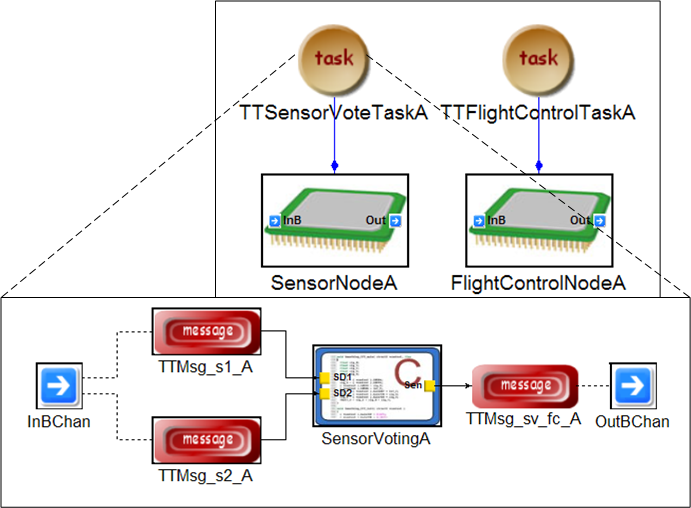
\includegraphics[width=0.55\columnwidth]{diagrams/tmr_deploy.png}
   \caption{Deployment model: task assignment to nodes and details of task definition.}
   \label{fig:tmr_deploy}
\end{figure}

A common graphical language captures the grouping of architecture components into tasks.  In ESMoL a task executes on a single processing node at a single periodic rate.  All components within the task execute synchronously.  Data sent between tasks takes the form of messages in the model.  Whether delivered locally (same processing node) or remotely, all inter-task messages are scheduled for delivery.  ESMoL uses logical execution time semantics found in time-triggered languages such as Giotto~\cite{henzinger01giotto} -- message delivery is scheduled after the deadline of the sending task, but before the release of the receiving tasks.  In the TT model of computation receivers assume that their data is available at task release time.  Tasks never block, but execute with whatever data is available each period.

Deployment concepts, tasks running on processing nodes and messages sent over data buses, are modeled as shown in Fig. \ref{fig:tmr_deploy}.  Most of the model elements shown here are actually references to elements defined in the architecture and platform models.  Model interpreters generate platform-specific code and analysis artifacts directly from the deployment models.

%%% OLD STUFF %%%%%%%%%%%%%%%%%%%%%%%%%%%%%%%%%%%%%%%%%%%%%%%%%%%%%%%%%%%%%%%%%%%%%%%%%%%%%



%\subsection{Code generators and synthesis tools}
%Model-based development is a high-level activity, i.e. programming with models instead of an algorithmic language. Therefore we need to generate executable code from the models. With proper infrastructure the generator could be more than just a model-to-code translator; it could be a code 'synthesizer' yielding low-level code from higher-level specifications. Synthesis differs from translation as it may search during the code generation process. For instance, on platforms with fixed-point arithmetic, the synthesizer could determine appropriate scaling factors for each operational step in a dataflow model based on known value ranges for inputs and outputs and the available fixed-point precision.

%Generating code from dataflow and Statechart models is a well-defined and solved problem, and there are many actual implementations. Code synthesis from higher-level models, however, is an active area of research with many open questions regarding code efficiency and correctness.

%\subsection{Verification and analysis}
%Verification and analysis are an inseparable part of the development process for high-confidence systems. There are many well-known verification techniques and tools; however, we must stress two concerns here: (1) verification tools often operate on models (i.e. abstractions of the system), not on detailed code and (2) verification results are meaningful only if model transformations from design models into analysis models or into code are correct: Properties must be carried over by the transformation with no addition of any artifacts extending behavior of the generated code beyond that of the model.

%Verification of model translators and construction of verification-based tools is an active area of research. Correctness of a model transformations is a very complex problem, but some early results indicate promising directions \cite{ananth:2006}: instead of proving correctness for a transformation in general, one can show that a particular instance of a transformation preserves the properties of interest and conclude that the properties hold for the input of the transformation.

%Another promising direction is a connection between models and the generated code. We are working on extending the code generator to carry forward model-level information to the generated code (as annotations) that provide help for the code-level verifier to check model-level properties on the code. This connection could potentially be used to improve performance, as the verifier could reason using higher-level abstractions than those immediately available from the code.  Other relevant work includes distributed modeling and verification tools like BIP~\cite{BasuBozgaSifakis07}, which strives for separation of concerns using a layered behavior model.
